\documentclass[11pt, a4paper]{article}
\usepackage[english]{babel}
\usepackage[utf8x]{inputenc}
\usepackage{amsmath}
\usepackage{graphicx}
\usepackage[colorinlistoftodos]{todonotes}
\usepackage{tikz, pgfplots, pgfplotstable}
\usepackage{float}
\usepackage{amssymb}
\pgfplotsset{compat=1.14}
\usepackage{subcaption}
\usepackage{multicol}
\captionsetup{compatibility=false}
\setlength{\marginparwidth}{2cm}
\setcounter{MaxMatrixCols}{14}
\usepackage{mathtools}
\DeclarePairedDelimiter\floor{\lfloor}{\rfloor}

\begin{document}

\begin{titlepage}

\newcommand{\HRule}{\rule{\linewidth}{0.5mm}} % Defines a new command for the horizontal lines, change thickness here

\center % Center everything on the page
 
%----------------------------------------------------------------------------------------
%	HEADING SECTIONS
%----------------------------------------------------------------------------------------

\textsc{\LARGE Ghent University}\\[1.5cm] % Name of your university/college
\textsc{\Large Applied Electromagnetism}\\[0.5cm] % Major heading such as course name
\HRule \\[0.4cm]
{\Huge Scattering from dielectric objects with the FDTD method}\\[0.5cm] % Minor heading such as course title
\HRule \\[1.5cm]

%----------------------------------------------------------------------------------------
%	TITLE SECTION
%----------------------------------------------------------------------------------------
 
%----------------------------------------------------------------------------------------
%	AUTHOR SECTION
%----------------------------------------------------------------------------------------

\begin{minipage}{0.60\textwidth}
\begin{center} \large
Paul \textsc{De Smul}\\
Thijs \textsc{Paelman}\\
Flor \textsc{Sanders}\break
\newline
Prof. dr. ir. Dries Vande Ginste\\
ir. Pieter Decleer\\
ir. Dries Bosman\break
\end{center}
\end{minipage}

%----------------------------------------------------------------------------------------
%	DATE SECTION
%----------------------------------------------------------------------------------------
{\large 2019-2020}\\[2cm] % Date, change the \today to a set date if you want to be precise

\vfill % Fill the rest of the page with whitespace

\end{titlepage}

\paragraph{\Large Project Applied Electromagnetism:\\\\Scattering from dielectric objects with the FDTD method}

\section{Introduction}

In this project we implemented a 2D-variant of the FDTD method, compatible with the inclusion of line sources with different profiles and several rectangular dielectric objects, as per the instruction paper made available to us.

The contributions of each group member were:
\begin{itemize}
    \item Paul De Smul: Implementation of supporting classes such as those for dielectrics, sources and the making of graphs; generation and analysis of results for simulations including dielectrics; researching accuracy versus efficiency trade-off; writing part of the report.
    \item Thijs Paelman: Implementation of dialog wrapper for interaction with the program; code validation using the Hankel function;  analysis of results; researching the courant limit; writing part of the report.
    \item Flor Sanders: Implementation of the FDTD-algorithm and its supporting space class; generation and analysis of results for simulations including dielectrics; researching the transmission coefficient at normal incidence; researching the influence of PEC boundaries; Remaining oversight of the project; writing part of and making final edits to the report.
\end{itemize}

\section{Method: implementation and usage}

\subsection{Implementation} % Flor
While all details of the workings of FDTD are described in the instruction paper, we will briefly add the specifics of our implementation in this section.

FDTD uses finite differences between the field values at certain fixed (discrete) positions to approximate the time derivatives (and thus differences) in those field values, based on Maxwell's equations. From these an iterative update algorithm can be derived. The discretization of the fields in space and time are visualized in figure \ref{Discretization}.

\begin{figure}[H]
\centering
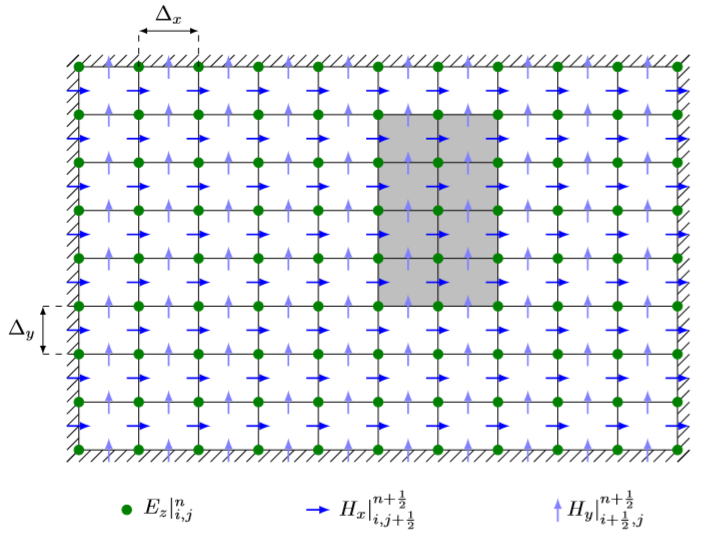
\includegraphics[width=0.6\linewidth]{Discretrization.PNG}
\caption{Discretization in space and time of the simulation domain}
\label{Discretization}
\end{figure}

\begin{equation}
    H_y|_{i+\frac{1}{2},j}^{n+\frac{1}{2}} = H_y|_{i+\frac{1}{2},j}^{n-\frac{1}{2}} + \frac{\Delta_t}{\mu_0 \Delta_x} \left( E_z|_{i+1,j}^{n} - E_z|_{i,j}^{n} \right)
\end{equation}

\begin{equation}
    H_x|_{i,j+\frac{1}{2}}^{n+\frac{1}{2}} = H_x|_{i,j+\frac{1}{2}}^{n-\frac{1}{2}} - \frac{\Delta_t}{\mu_0 \Delta_y} \left( E_z|_{i,j+1}^{n} - E_z|_{i,j}^{n} \right)
\end{equation}

\begin{equation}
\begin{split}
    E_z|_{i,j}^{n+1} = & E_z|_{i,j}^{n} + \frac{\Delta_t}{\epsilon_0 \epsilon_r \Delta_x} \left( H_y|_{i+\frac{1}{2},j}^{n+\frac{1}{2}} - H_y|_{i-\frac{1}{2},j}^{n+\frac{1}{2}} \right) \\
    & - \frac{\Delta_t}{\epsilon_0 \epsilon_r \Delta_x} \left( H_x|_{i,j+\frac{1}{2}}^{n+\frac{1}{2}} - H_x|_{i,j-\frac{1}{2}}^{n+\frac{1}{2}} \right) - \frac{\Delta_t}{\epsilon_0 \epsilon_r \Delta_x \Delta_y} I|_{i,j}^{n+\frac{1}{2}}
\end{split}
\end{equation}

We decided to represent our field values, as well as the dielectric properties of the space in 2D numpy arrays, in which the dimensions represent the index index along x-axis ($i = x(-1/2)/\Delta_x$) and index along y-axis ($j = y(-1/2)/\Delta_y$) (With the term -1/2 in i for the $H_y$ component, in j for the $H_x$ component). The time-index ($n = t(-1/2)/\Delta_t$) is taken into account by performing above update equations in a for loop with n iterations (With the term -1/2 in n for both $H$ field components). 

The update equations can then be directly implemented for the whole (inner) field by slicing the arrays in the correct ways and applying above equations to them. Finally, measurements for the field values can be obtained by saving the values at the correct indices for any position in the box at every iteration.

One difficulty we stumbled upon during implementation was how to define the material parameter $\epsilon_r$ at the points for which the $E_z$ values are kept. As can be seen in figure \ref{Discretization}, these points coincide with the corners of the discrete units of space, which might have different values of $\epsilon_r$. Because of the staggered discretization of space, material borders are ill defined, this is a clear disadvantage of the FDTD method. We came up with the following two solutions:
\label{eps_averaging_subsection}
\begin{enumerate}
    \item \label{eps_averaging} Average out $\epsilon_r$ over the surrounding units of space. \\
    This option is the most obvious one, but results in values $\epsilon_r$ which were not present in the original problem description.
    \item Move the dielectric object by a half step in relation to the space grid. \\
    Since there's no magnetic contrast ($\mu = \mu_0, \forall \text{ } (x,y) $ in the box), we can easily solve this issue by moving the dielectric object by $\pm \Delta_x/2$ and $\pm \Delta_y/2$.
\end{enumerate}

In the end, we decided to implement both options and add an optional argument in the FDTD-simulation function where the user can decide whether averaging is used or not. If the resolution is sufficiently high, both options should yield the same (or at least very similar) results. For consistency, we decided to always use the second option in our simulations.

\subsection{Usage} % Thijs

For all simulations performed in the next sections, we wrote a script holding the variables and performing the necessary operations. For quick generation of results on the other hand, we made an input wrapper around the bare simulation code. The most important things to take into account before starting are:
\begin{itemize}
    \item Are all necessary python3 libraries installed? We assume so. These are: \emph{numpy}, \emph{scipy}, \emph{matplotlib} and for certain of our scripts \emph{timeit}.
    \item All the files of our project should be in the same directory.
    \item Run \emph{main.py} with python3. The interaction will be textual.
\end{itemize}{}
Once you started the program, it should be self explanatory, but for convenience will give a quick walkthrough here. We'll just state what will be asked and in which order, but first a few \textbf{warnings}.
All the input values have to be numbers, in certain cases integers. To enter a floating point number like $1.23\cdot10^{-67}$, you'll have to use the following format: 1.23e-67.
Furthermore: if you make a mistake in the input, like using a comma (,) instead of a dot (.) or filling in e-67 instead of 1e-67, a ValueError will be thrown and you'll have to start over.
Last remark: we do not test if the given parameters make sense, so that's up to you.

\newpage
\begin{enumerate}
    \item Dimensions of the simulation domain, namely width (x-axis), length (y-axis) and duration.
    \item The parameters of all the dielectric objects. See figure \ref{fig:dielec_axis} for the used conventions.
    \begin{figure}[H]
        \centering
        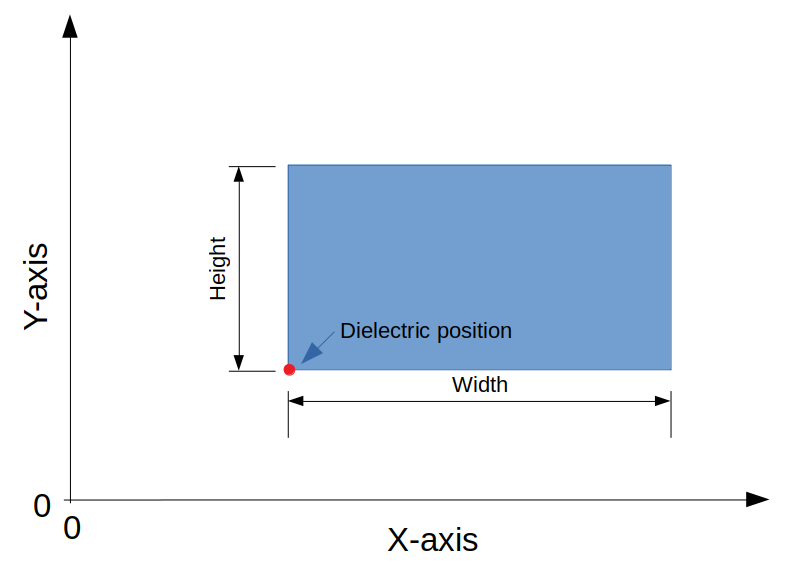
\includegraphics[width=0.5\linewidth]{fig/dielectric_axis.png}
        \caption{Used conventions within our program}
        \label{fig:dielec_axis}
    \end{figure}
    \item If $\epsilon_r$ should be averaged out (see section \ref{eps_averaging_subsection}, listitem \ref{eps_averaging}).
    \item The line source: position, current profile with two choices, namely the \emph{Gaussian pulse} and the \emph{Gaussian-modulated sinusoidal radio-frequency pulse}. After your choice, the pulse parameters are requested.
    \item Thereafter, the space discretization is asked, for which a range of recommended values is offered.
    \item Next up is the time discretization, for which a maximum recommended value is given (see courant limit).
    \item Following are the coordinates of the measurement points.
    \item Last is an option to visualize the fields during the simulation. We used this to interpret some of the results and we don't want to withhold this from you. You can enter after how many seconds the simulation shows an intermediate situation, giving a color plot with a qualitative situation of the amplitude for the $E$ and $H$ fields (so no numbers). You have to close the plots to continue the simulation!
\end{enumerate}

After all the parameters are inputted, a visualisation of the space is given to quickly check if everything seems like intended. Different relative permittivities get a different color, but no numbers are given.
When you close this window, the effective simulation will run and when finished, the graphs will show up. We encourage you to always maximize the window, to ensure good typesetting.
You have to close each graph to get the next, at which moment they will be saved in .png format in the plots folder.

First, the source current is plotted in function of time.
Thereafter, for each measurement point are $H_x$, $H_y$ and $E_z$ plotted. There can be 2 vertical lines on these graphs. The first one represents the time for the wave to arrive from the source and the second represents the time for the first reflection to arrive. These are estimations using the speed of light in \textbf{vacuum} and the assumption that the source starts radiating at $t = 0$. These are therefore merely guidelines!


\section{Simulations: numerical results and analysis}

\subsection{Code validation using the Hankel function} \label{hankel} % Thijs

To validate our code, we will compare the results it generates with the analytical results for an elementary line source with purely sinusoidally varying current density in the frequency domain. The setup is simply free space. A visualisation of the source and measurement points locations is given in figure \ref{fig:visual_code_validation}. The space is in this case a square with side $200 m$, with the source right in the middle.

\begin{figure}[H]
    \centering
    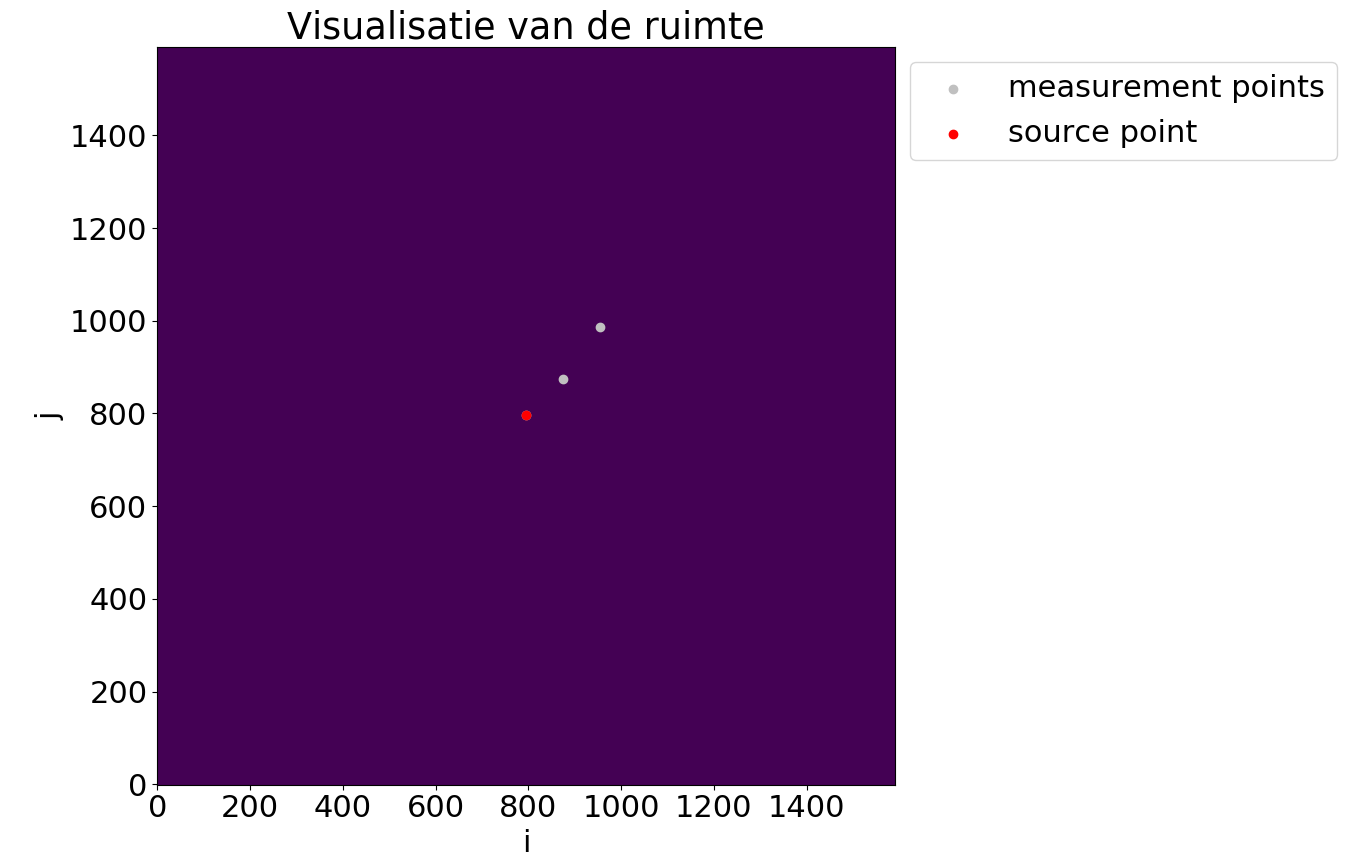
\includegraphics[width=0.95\linewidth]{fig/em_vis_hankel.png}
    \caption{Visualisation of the space used for code validation}
    \label{fig:visual_code_validation}
\end{figure}

In first instance, we compared the amplitude of our experimental results with those of the Hankel function for both locations, the resulting plots can be found in figures \ref{fig:abs_code_validation} and \ref{fig:abs_code_validation}. As can be seen in these figures, the amplitudes of the theoretical and experimental results are very much alike.

Next the phases of both results were compared. At first instance, when using the analytical spectrum of the source (see instruction paper) the phases didn't seem to line up. The cause of this was that we were comparing an experimental time-shifted signal with an analytical signal without a time-shift, thus losing all phase information. To overcome this problem, we simply performed a Fourier transform on the experimental signal for the phase comparison. The final results for the phase comparison are shown in figure \ref{fig:phase_code_validation_2}.

\begin{figure}[H]
    \centering
    \begin{subfigure}{\textwidth}
        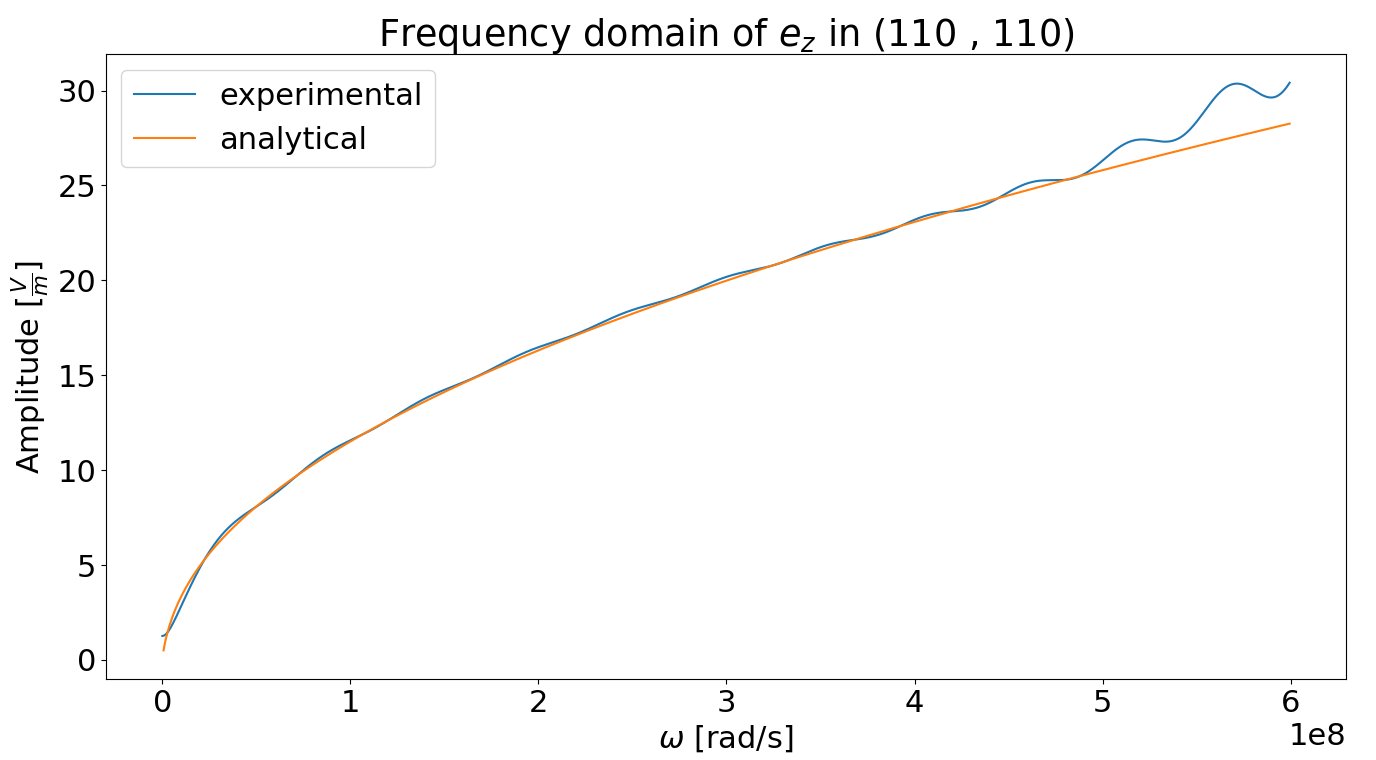
\includegraphics[width=0.95\linewidth]{fig/em_abs_hankel.png}
        \caption{point 1 (coordinates in m)}
        \label{fig:abs_code_validation}
    \end{subfigure}
    \begin{subfigure}{\textwidth}
        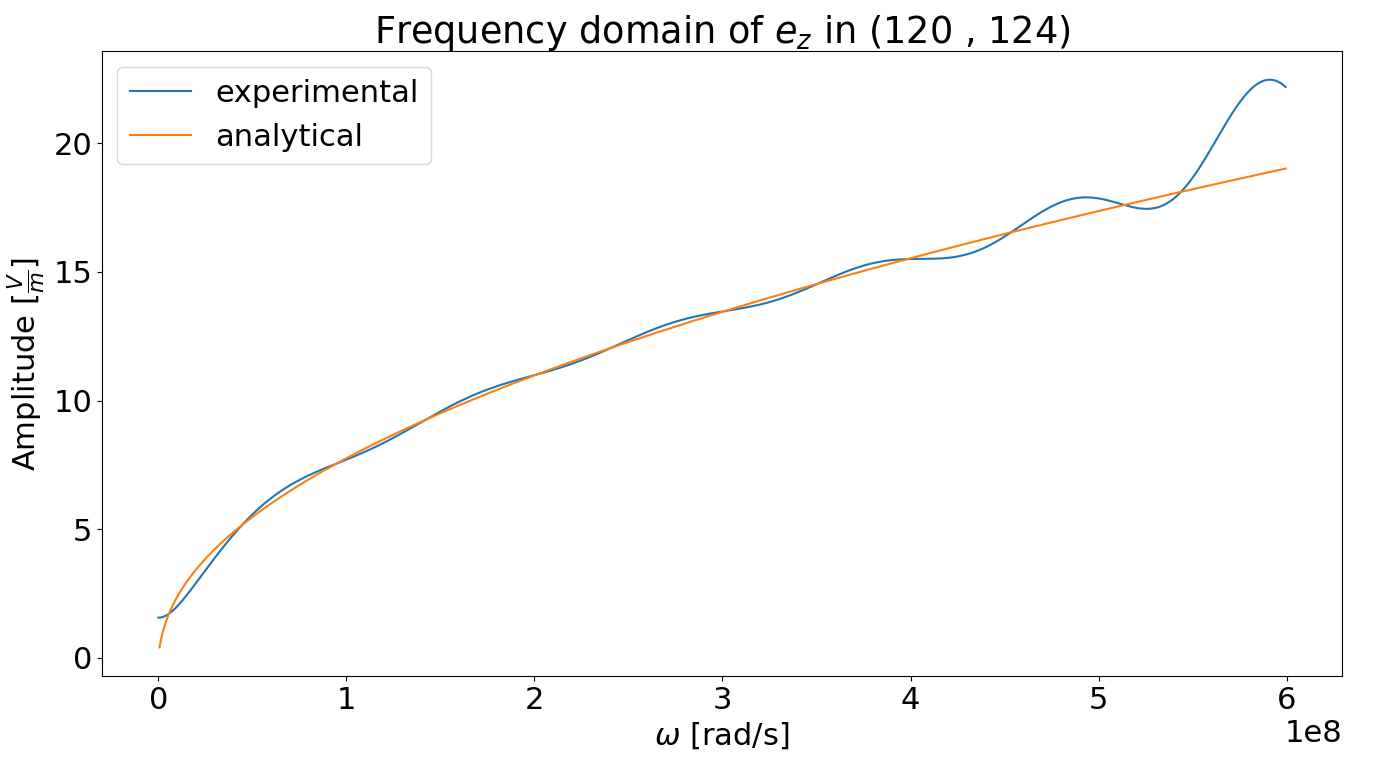
\includegraphics[width=0.95\linewidth]{fig/em_abs_hankel_point_2.png}
        \caption{point 2 (coordinates in m)}
        \label{fig:abs_code_validation_2}
    \end{subfigure}
    \caption{Comparing the analytical with the experimental amplitude of the electric field in the frequency domain}
\end{figure}
\begin{figure}[h]
    \centering
    \begin{subfigure}{\textwidth}
        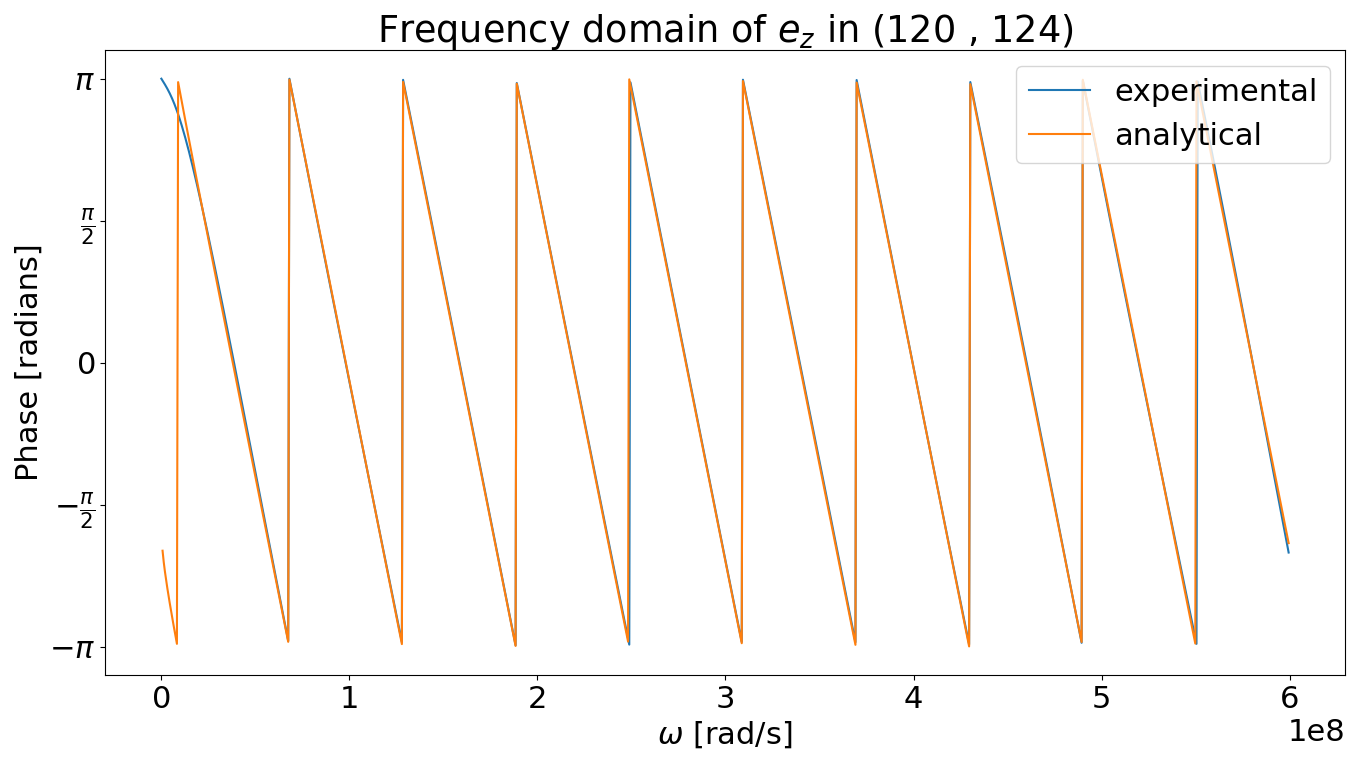
\includegraphics[width=0.95\linewidth]{fig/phase_hankel_2.png}
        \caption{point 2 (coordinates in m)}
        \label{fig:phase_code_validation_2}
    \end{subfigure}
    \caption{Comparing the analytical with the experimental phase of the electric field in the frequency domain}
\end{figure}

\newpage
\subsection{Inclusion of sources and dielectrics} % Paul

\subsubsection{Transmission and reflection for a single dielectric}
The first experiment we considered was a setup of two half-spaces (each with dimensions $w=75 cm$ by $l=150 cm$), with one half being free space and another half being filled up by a dielectric material, with a relative permittivity $\epsilon_r = 4$. In this space we place a current point source with a Gaussian pulse profile ($J_0 = 1 A$, $\sigma = 0.1 ns$, $t_c = 0.4 ns$) in free space at distance $d = 20 cm$ from the plane interface. A visualization of the space is given in figure \ref{hs_vis}.

We proceeded to measure the magnetic and electric fields both in free space and in the dielectric, both at $d=20cm$ from the plane interface. The discretization parameters were calculated as follows:
\begin{itemize}
    \item $\lambda_{min} = 2 \pi c \cdot \sigma/(3\sqrt{\epsilon_r}) = 3.14 cm$
    \item $\Delta_x = \Delta_y = \lambda_{min}/25 = 1.26 mm$
    \item $\Delta_t = \left( 3c \sqrt{1/\Delta_x^2 + 1/\Delta_y^2} \right)^{-1} = 98.7 ps$
\end{itemize}

\begin{figure}[H]
    \centering
    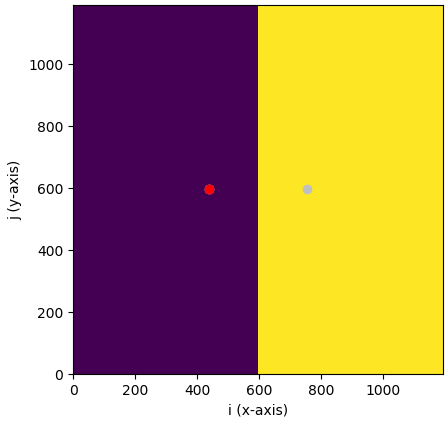
\includegraphics[width=0.6\linewidth]{halfspace/halfspace_viz.png}
    \caption{Visualisation of the simulation space}
    \label{hs_vis}
\end{figure}

The measurements for the fields in free space are shown in figure \ref{hs_source}. In the leftmost part of the graphs, the electric and magnetic fields as a direct result of the source current can be seen.

In theory, when using a line source with a Dirac-current profile, these field values should be infinitely large when measured at the source position. However, because FDTD divides the space into finite squares this isn't the case, since the current gets averaged out as a finite current density over such an elementary surface.

To inspect the reflections coming from the dielectric material we need to zoom in on the little bumps around $1.8 ns$, the resulting graphs are shown in figure \ref{hs_source_zoom}. 

First off, we notice that the magnetic field only has a non-zero component in the y direction. This can easily be explained using Ampere's law around a current line source, which results in a magnetic field with only a component along the azimuthal unit vector. This means the magnetic and electric field are completely tangential to the plane interface for normal incidence.

Furthermore we notice that the $E_z$ field is inverted after reflection, but the $H_y$ field is not. This can be explained by analysing the situation for plane waves impeding upon a plane interface under normal incidence, for which the same happens.

Finally, the field measurements in the dielectric are shown in figure \ref{hs_diel}. 

The $E_z$ and $H_y$ field have the same sign as the original wave as expected, again comparing with the situation for impeding plane waves.

Both the reflected and transmitted wave have greatly reduced amplitudes. Not only has the amplitude decreased because of the distance the waves have traveled, but also because when the original wave is split at the boundary of the dielectric material into a reflected and transmitted wave, the energy of that wave is distributed between the two. The ratio of this division is dependent on the permittivity of the dielectric material and is further investigated in the next section.   

\begin{figure}[H]
    \centering
    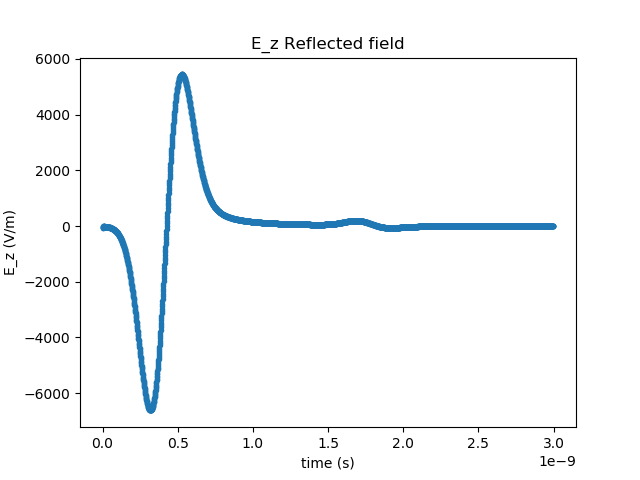
\includegraphics[width=0.49\linewidth]{halfspace/Ezr.png}
    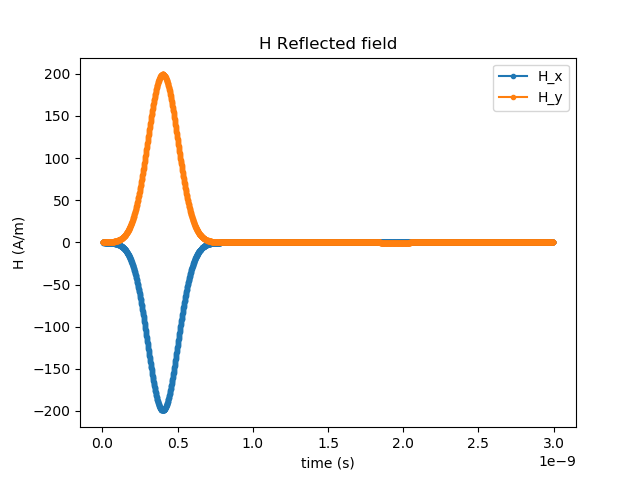
\includegraphics[width=0.49\linewidth]{halfspace/Hxyr.png}
    \caption{Fields measured at source position}
    \label{hs_source}
\end{figure}

\begin{figure}[H]
    \centering
    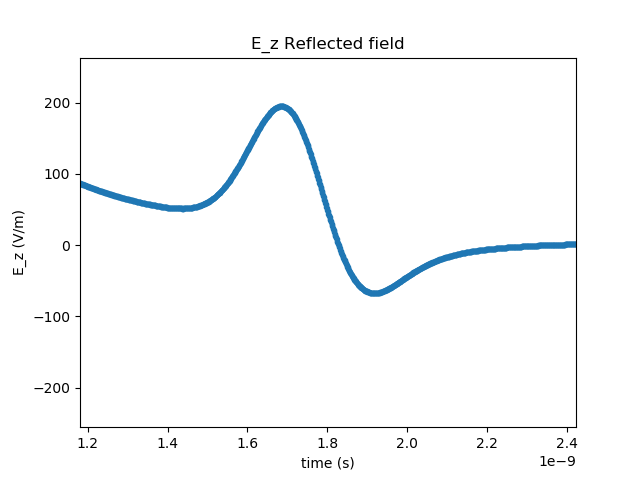
\includegraphics[width=0.49\linewidth]{halfspace/Ezrzoom.png}
    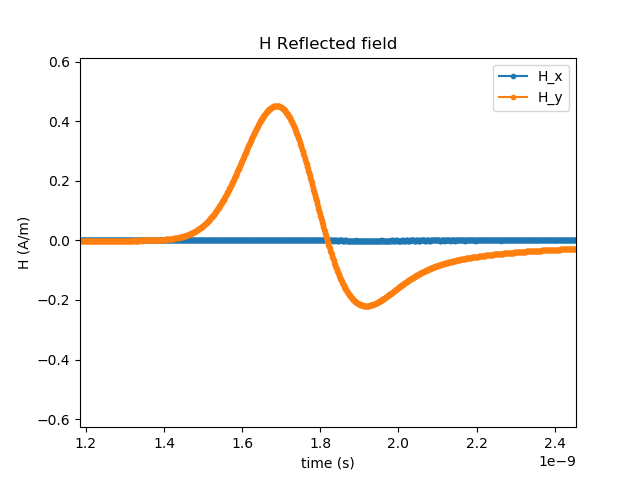
\includegraphics[width=0.49\linewidth]{halfspace/Hxyrzoom.png}
    \caption{Reflected fields measured at source position}
    \label{hs_source_zoom}
\end{figure}

\begin{figure}[H]
    \centering
    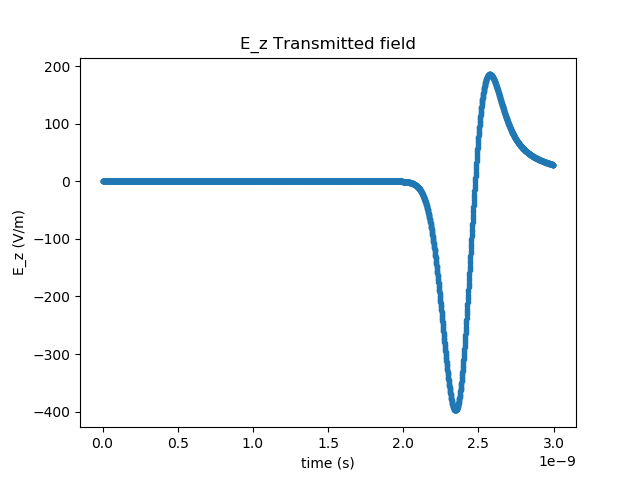
\includegraphics[width=0.49\linewidth]{halfspace/Ezt.png}
    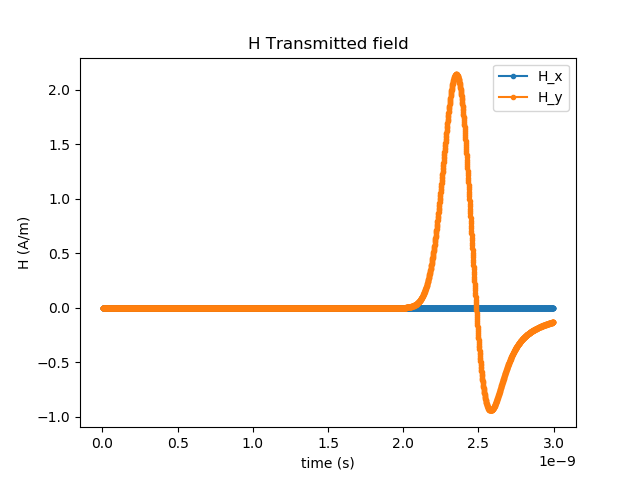
\includegraphics[width=0.49\linewidth]{halfspace/Hxyt.png}
    \caption{Transmitted fields in dielectric material}
    \label{hs_diel}
\end{figure}

\subsubsection{Transmission coefficient at normal incidence}
In this section we will reuse a similar setup as in the previous one, albeit with slightly smaller dimensions to reduce computation time ($w=25 cm$, $h=50 cm$, $d=5cm$), we will also consider the setup for a range of different values for the relative permittivity of the dielectric ($\epsilon_r = 1 \text{ to } 20$). 

It proved to be especially hard in this case to completely separate the reflected wave from the origin wave, so we decided to only discuss the waves transmitted into the dielectric for this part, both qualitatively and quantitatively.

Plotting the transmitted electric wave profiles for different values of $\epsilon_r$ results in figure \ref{T_fields}.

\begin{figure}[H]
    \centering
    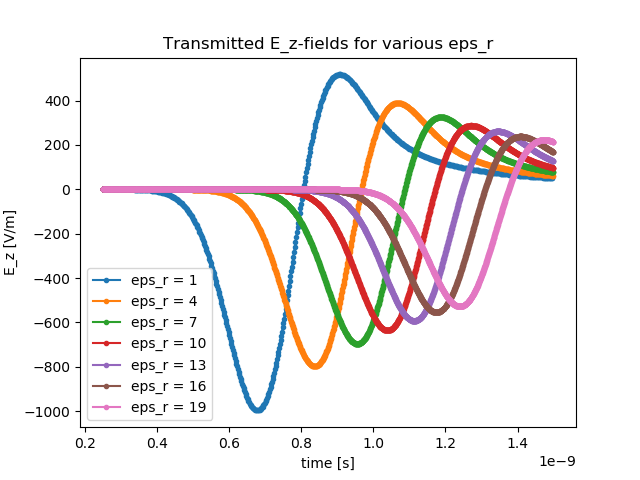
\includegraphics[width=0.75\linewidth]{transmission/E_z_t_eps_r.png}
    \caption{Transmitted fields in dielectric material}
    \label{T_fields}
\end{figure}

We can immediately draw two obvious conclusions from this graph:
\begin{itemize}
    \item As $\epsilon_r$ increases, the transmitted wave takes longer to reach our measurement point. This makes a lot of sense, since the speed of light in a non-magnetic medium is determined by $v=c/\sqrt{\epsilon_r}$, hence the speed of the wave will decrease as the permittivity of the material increases. 
    \item As $\epsilon_r$ increases, the amplitude of the transmitted wave decreases. This is extremely logical since for higher $\epsilon_r$ a bigger part of the wave is reflected when reaching the dielectric surface.
\end{itemize}

We decided to explore this last result in a little more detail. In our courses, we derived the following equation to determine the transmission coefficient of a plane wave for normal incidence upon a plane interface between two homogeneous, linear, isotropic and infinitely extending media:

\begin{equation}
    T_n = \frac{2z_{c2}}{z_{c1}+z_{c2}} = \frac{2}{1+\sqrt{\epsilon_r}},  (z_{c1}=z_{c0} \text{ and } z_{c2}=\frac{z_{c0}}{\sqrt{\epsilon_r}})
\end{equation}

By normalizing the amplitudes of the transmitted fields with respect to the amplitude received for complete transmission ($\epsilon_r = 1$), we can experimentally obtain the transmission coefficients for our setup. The resulting graph is shown in figure \ref{T_coefficients}.

\begin{figure}[H]
    \centering
    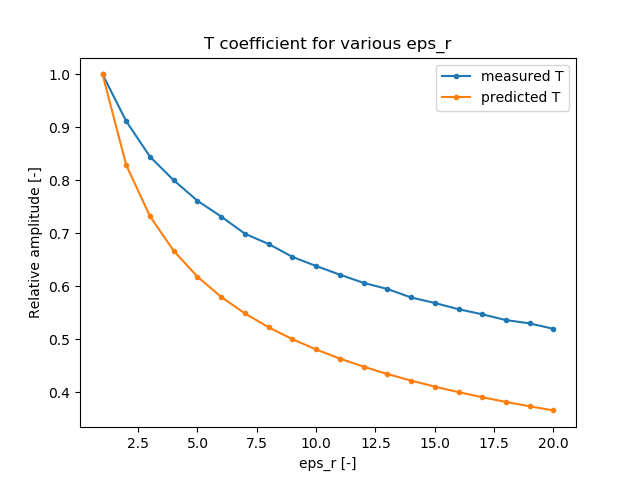
\includegraphics[width=0.75\linewidth]{transmission/TRcoeff_eps_r.png}
    \caption{Transmission coefficients for various $\epsilon_r$}
    \label{T_coefficients}
\end{figure}

While qualitatively following a similar trend, there is a significant deviation between the experimentally obtained results and those from the equation. The reason for this is that in proposing above equation, we made the assumption that our impeding wave can be approximated as an infinitely extending plane wave. This is obviously not an accurate approximation, the distance between the point source and the plane interface is way too small to be able to neglect the curvature of the circular wave-front. 

\subsection{Accuracy versus efficiency trade-off} % Flor & Paul
To evaluate the efficiency of our simulation, we will use the python \emph{timeit} library to time our code. There is some random variation on the timings as the computer is doing other stuff in the background so we will run 5 simulations for every value of $\omega_{max}$ and take the average value. We will give $\lambda_{min}$, $\Delta_x$ and $\Delta_t$ as our measure of accuracy.

The simulations were done on an empty square space with length $1m$, no dielectrics and in the middle a line source with the same profile as used in the previous two sections for a simulation time of $2 ns$.

\begin{center}
\begin{tabular}{ c c c c c} 
 $\omega_{max}$ & Avg runtime (s) & $\lambda_{min}$ (m) & $\Delta_x$ & $\Delta_t$ \\
 2/$\sigma$ & 1.42 & 0.094 & $3.77\cdot10^{-3}$ & $2.96\cdot10^{-12}$\\ 
 3/$\sigma$ & 6.27 & 0.063 & $2.51\cdot10^{-3}$ & $1.97\cdot10^{-12}$\\ 
 4/$\sigma$ & 16.7 & 0.047 & $1.88\cdot10^{-3}$ & $1.48\cdot10^{-12}$\\ 
 5/$\sigma$ & 31.5 & 0.038 & $1.51\cdot10^{-3}$ & $1.18\cdot10^{-12}$
\end{tabular}
\end{center}

As can be seen in the results, a larger estimation for the maximum bandwidth of our pulse results in a more precise grid for both the space and time domain discretizations. Due to the use of the courant limit (which is investigated in the next section), precision is won in all three dimensions simultaneously. The price paid for this is an sharp increase in average simulation runtime.

We conclude that within reasonable boundaries (see courant limit), the space and time steps can be chosen depending on how accurate the results need to be and that by allowing coarser estimations the total simulation time can be significantly improved.

\subsection{Courant limit}

To investigate the Courant limit, we used the same setup as in section \ref{hankel}, however halving the sides of the space to reduce simulation time. 

To see what happens when we take a time step larger than the Courant limit, we set $\Delta t = \text{Courant limit} \cdot 1.0001$.

Like you can see on figures \ref{fig:courant_lin} and \ref{fig:courant_log}. At first everything goes well, but after a while the measurement starts growing exponentially, consistently over- and undershooting the changes needed to be made to obtain valid results.

In conclusion: to obtain valid results, it is extremely important that the Courant limit is satisfied.

\begin{figure}[H]
    \centering
    \begin{subfigure}{\textwidth}
        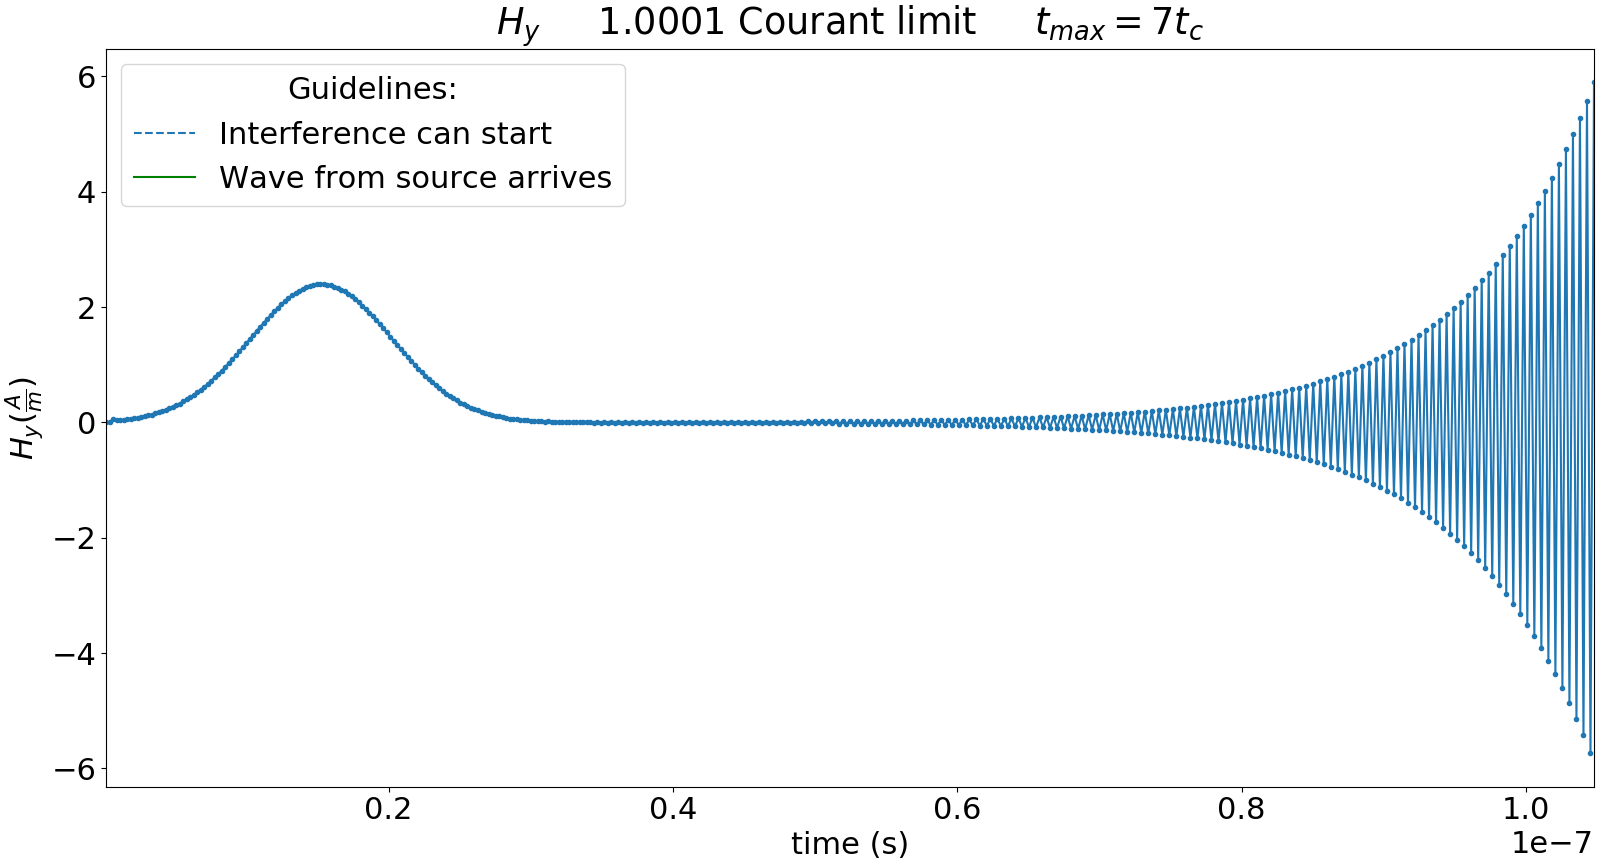
\includegraphics[width=0.95\linewidth]{fig/courant_lin.png}
        \caption{Linear plot}
        \label{fig:courant_lin}
    \end{subfigure}
    \begin{subfigure}{\textwidth}
        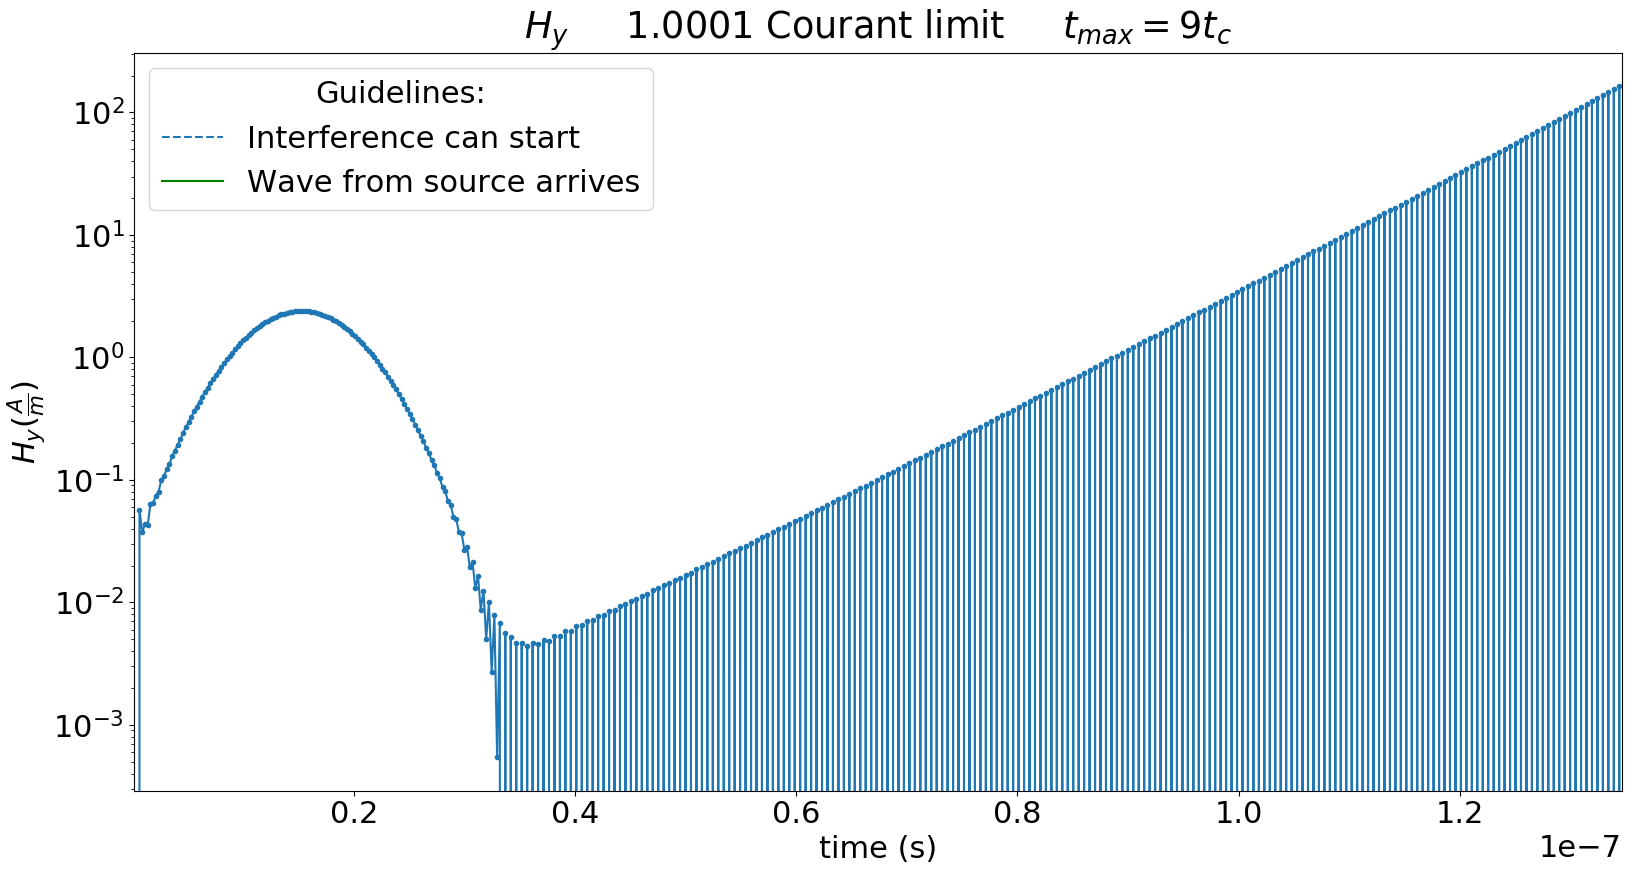
\includegraphics[width=0.95\linewidth]{fig/courant_log.png}
        \caption{Logarithmic plot}
        \label{fig:courant_log}
    \end{subfigure}
    \caption{Simulations with $\Delta t = 1.0001 \cdot$ Courant limit}
\end{figure}

\subsection{Influence of PEC boundaries} % Flor

To investigate the influence of the PEC boundaries surrounding our box, we will use a Gaussian pulse current source at the center of our space with dimensions $35 cm$ by $35 cm$, the profile of which is shown in figure \ref{PEC_reflection_source}. We let the simulation run and obtain the measurement for the electric field at the source, which is shown in figure \ref{PEC_reflection_field}.

There are two distinct regions to be separated in this graph. The first part (left of the dashed line) shows the electric field pulse as a direct result of the source current. The second part (right of the dashed line) shows the field pulses as a result of the reflections of the electric field of the PEC boundaries.

If we would allow these reflected waves to interfere with our measurements, it would be incredibly hard to interpret our results. To avoid this we made sure to stop our simulations well before the reflection waves hit for our simulations in the previous sections.

\begin{figure}[H]
\centering
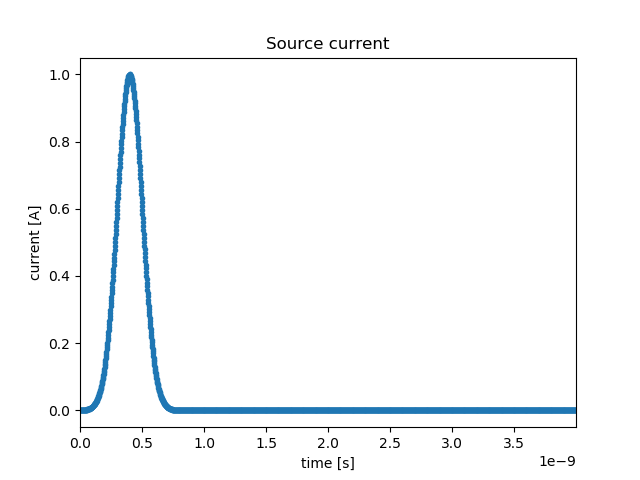
\includegraphics[width=0.75\linewidth]{PEC/PEC_current.png}
\caption{Gaussian pulse source with $J_0=1 A/m^2$, $\sigma=0.1 ns$, $t_c = 0.4 ns$}
\label{PEC_reflection_source}
\end{figure}

\begin{figure}[H]
\centering
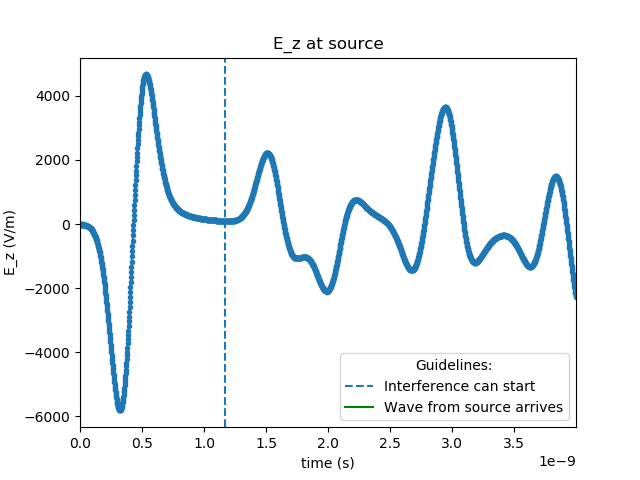
\includegraphics[width=0.75\linewidth]{PEC/PEC_E_z.png}
\caption{$E_z$ field measured at source}
\label{PEC_reflection_field}
\end{figure}


\end{document}
